% Auto: scripts/66_credit_forest_plot.py
\begin{figure}[tbp]
\centering
\resizebox{\textwidth}{!}{%
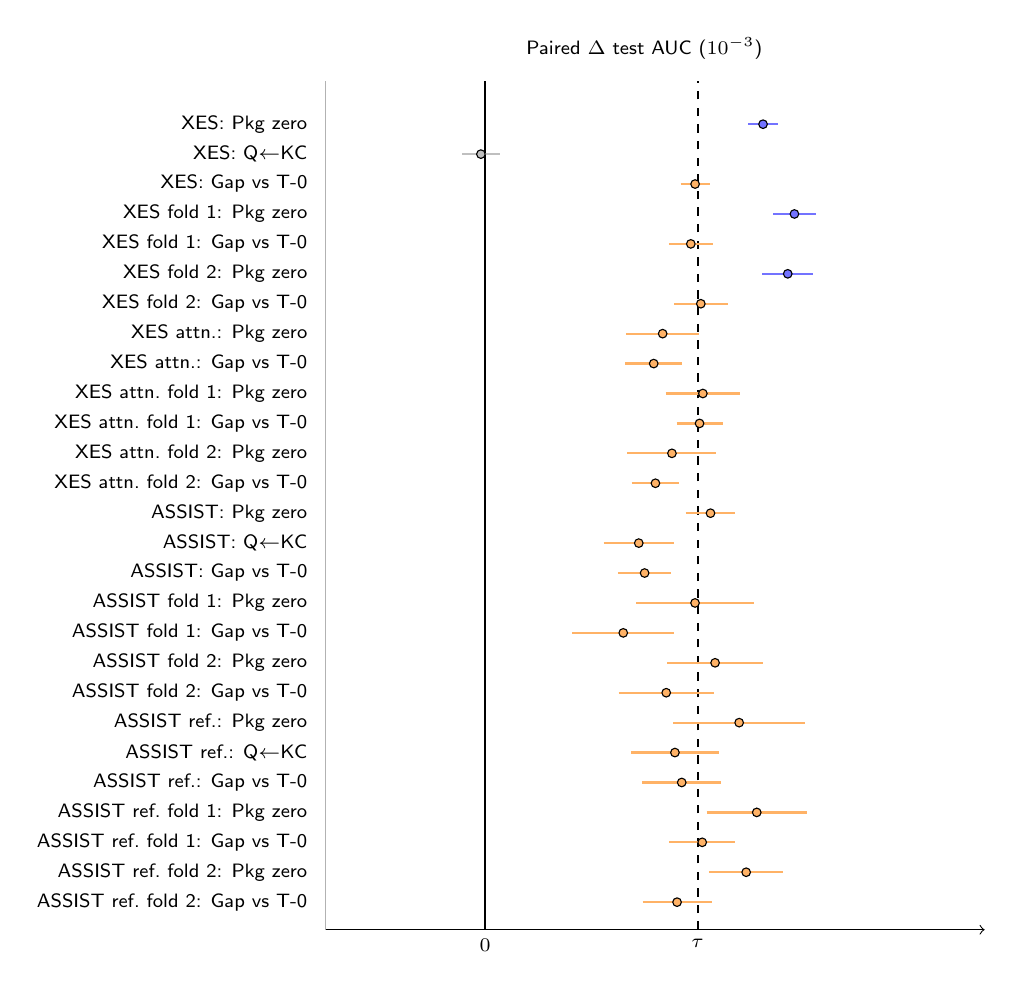
\begin{tikzpicture}[x=1.35cm,y=1cm,font=\scriptsize\sffamily]
\draw[gray!60] (-1.5,-0.35) -- (-1.5,10.430000000000001);
\draw[thick] (0,-0.35) -- (0,10.430000000000001);
\draw[thick,dashed] (2,-0.35) -- (2,10.430000000000001);
\node[below] at (0,-0.35) {$0$};
\node[below] at (2,-0.35) {$\tau$};
\node[above] at (1.5,10.58) {Paired $\Delta$ test AUC ($10^{-3}$)};
\draw[blue!55, thick] (2.477626811869569,9.88) -- (2.753263090827446,9.88);
\node[draw, circle, fill=blue!55, inner sep=1.1pt] at (2.615444951351953,9.88) {};
\node[anchor=east, align=right] at (-1.58,9.88) {XES: Pkg zero};
\draw[gray!50, thick] (-0.21519072881740237,9.5) -- (0.13759144505934162,9.5);
\node[draw, circle, fill=gray!50, inner sep=1.1pt] at (-0.038799641874620594,9.5) {};
\node[anchor=east, align=right] at (-1.58,9.5) {XES: Q$\leftarrow$KC};
\draw[orange!60, thick] (1.840079820136517,9.120000000000001) -- (2.112684761022292,9.120000000000001);
\node[draw, circle, fill=orange!60, inner sep=1.1pt] at (1.9763822905828121,9.120000000000001) {};
\node[anchor=east, align=right] at (-1.58,9.120000000000001) {XES: Gap vs T-0};
\draw[blue!55, thick] (2.7117952415929896,8.74) -- (3.1096619915191934,8.74);
\node[draw, circle, fill=blue!55, inner sep=1.1pt] at (2.9107286165610646,8.74) {};
\node[anchor=east, align=right] at (-1.58,8.74) {XES fold 1: Pkg zero};
\draw[orange!60, thick] (1.7296690999984503,8.360000000000001) -- (2.1423061911775587,8.360000000000001);
\node[draw, circle, fill=orange!60, inner sep=1.1pt] at (1.9359876455931624,8.360000000000001) {};
\node[anchor=east, align=right] at (-1.58,8.360000000000001) {XES fold 1: Gap vs T-0};
\draw[blue!55, thick] (2.606987750575301,7.98) -- (3.0887666175814585,7.98);
\node[draw, circle, fill=blue!55, inner sep=1.1pt] at (2.847877184084402,7.98) {};
\node[anchor=east, align=right] at (-1.58,7.98) {XES fold 2: Pkg zero};
\draw[orange!60, thick] (1.7780026630000918,7.6000000000000005) -- (2.282458555941833,7.6000000000000005);
\node[draw, circle, fill=orange!60, inner sep=1.1pt] at (2.030230609477268,7.6000000000000005) {};
\node[anchor=east, align=right] at (-1.58,7.6000000000000005) {XES fold 2: Gap vs T-0};
\draw[orange!60, thick] (1.3247754315369529,7.220000000000001) -- (2.017533504386136,7.220000000000001);
\node[draw, circle, fill=orange!60, inner sep=1.1pt] at (1.671154467970204,7.220000000000001) {};
\node[anchor=east, align=right] at (-1.58,7.220000000000001) {XES attn.: Pkg zero};
\draw[orange!60, thick] (1.3178512869055135,6.840000000000001) -- (1.8558600469546886,6.840000000000001);
\node[draw, circle, fill=orange!60, inner sep=1.1pt] at (1.5868556669368261,6.840000000000001) {};
\node[anchor=east, align=right] at (-1.58,6.840000000000001) {XES attn.: Gap vs T-0};
\draw[orange!60, thick] (1.6994649350120454,6.460000000000001) -- (2.3991327827354363,6.460000000000001);
\node[draw, circle, fill=orange!60, inner sep=1.1pt] at (2.0492988588824868,6.460000000000001) {};
\node[anchor=east, align=right] at (-1.58,6.460000000000001) {XES attn.\ fold 1: Pkg zero};
\draw[orange!60, thick] (1.8013793060570698,6.080000000000001) -- (2.23485467086112,6.080000000000001);
\node[draw, circle, fill=orange!60, inner sep=1.1pt] at (2.0181169884645134,6.080000000000001) {};
\node[anchor=east, align=right] at (-1.58,6.080000000000001) {XES attn.\ fold 1: Gap vs T-0};
\draw[orange!60, thick] (1.3391954319301742,5.700000000000001) -- (2.177616122388537,5.700000000000001);
\node[draw, circle, fill=orange!60, inner sep=1.1pt] at (1.7584057771698358,5.700000000000001) {};
\node[anchor=east, align=right] at (-1.58,5.700000000000001) {XES attn.\ fold 2: Pkg zero};
\draw[orange!60, thick] (1.3781821866149,5.32) -- (1.8281644625705957,5.32);
\node[draw, circle, fill=orange!60, inner sep=1.1pt] at (1.6031733245983726,5.32) {};
\node[anchor=east, align=right] at (-1.58,5.32) {XES attn.\ fold 2: Gap vs T-0};
\draw[orange!60, thick] (1.8862572823977792,4.94) -- (2.356318679104875,4.94);
\node[draw, circle, fill=orange!60, inner sep=1.1pt] at (2.1212879807572027,4.94) {};
\node[anchor=east, align=right] at (-1.58,4.94) {ASSIST: Pkg zero};
\draw[orange!60, thick] (1.1154863700325135,4.5600000000000005) -- (1.7773250995301888,4.5600000000000005);
\node[draw, circle, fill=orange!60, inner sep=1.1pt] at (1.4464057347896242,4.5600000000000005) {};
\node[anchor=east, align=right] at (-1.58,4.5600000000000005) {ASSIST: Q$\leftarrow$KC};
\draw[orange!60, thick] (1.2509524372847804,4.180000000000001) -- (1.7518181526209888,4.180000000000001);
\node[draw, circle, fill=orange!60, inner sep=1.1pt] at (1.5013852949591455,4.180000000000001) {};
\node[anchor=east, align=right] at (-1.58,4.180000000000001) {ASSIST: Gap vs T-0};
\draw[orange!60, thick] (1.4239715195457245,3.8000000000000007) -- (2.527421881252598,3.8000000000000007);
\node[draw, circle, fill=orange!60, inner sep=1.1pt] at (1.9756967004129544,3.8000000000000007) {};
\node[anchor=east, align=right] at (-1.58,3.8000000000000007) {ASSIST fold 1: Pkg zero};
\draw[orange!60, thick] (0.8195844392759375,3.420000000000001) -- (1.7813730280482927,3.420000000000001);
\node[draw, circle, fill=orange!60, inner sep=1.1pt] at (1.3004787336741375,3.420000000000001) {};
\node[anchor=east, align=right] at (-1.58,3.420000000000001) {ASSIST fold 1: Gap vs T-0};
\draw[orange!60, thick] (1.7149171542207795,3.040000000000001) -- (2.613716685620122,3.040000000000001);
\node[draw, circle, fill=orange!60, inner sep=1.1pt] at (2.164316919931686,3.040000000000001) {};
\node[anchor=east, align=right] at (-1.58,3.040000000000001) {ASSIST fold 2: Pkg zero};
\draw[orange!60, thick] (1.256675790479474,2.660000000000001) -- (2.1526027802800094,2.660000000000001);
\node[draw, circle, fill=orange!60, inner sep=1.1pt] at (1.704639285390941,2.660000000000001) {};
\node[anchor=east, align=right] at (-1.58,2.660000000000001) {ASSIST fold 2: Gap vs T-0};
\draw[orange!60, thick] (1.7716459081674834,2.280000000000001) -- (3.0099715347701252,2.280000000000001);
\node[draw, circle, fill=orange!60, inner sep=1.1pt] at (2.3908087214842833,2.280000000000001) {};
\node[anchor=east, align=right] at (-1.58,2.280000000000001) {ASSIST ref.: Pkg zero};
\draw[orange!60, thick] (1.3745769356789128,1.9000000000000004) -- (2.1986026602891937,1.9000000000000004);
\node[draw, circle, fill=orange!60, inner sep=1.1pt] at (1.7865897979943535,1.9000000000000004) {};
\node[anchor=east, align=right] at (-1.58,1.9000000000000004) {ASSIST ref.: Q$\leftarrow$KC};
\draw[orange!60, thick] (1.479260835451334,1.5200000000000014) -- (2.2217243265657793,1.5200000000000014);
\node[draw, circle, fill=orange!60, inner sep=1.1pt] at (1.8504925810178374,1.5200000000000014) {};
\node[anchor=east, align=right] at (-1.58,1.5200000000000014) {ASSIST ref.: Gap vs T-0};
\draw[orange!60, thick] (2.084314516499326,1.1400000000000006) -- (3.028039744772141,1.1400000000000006);
\node[draw, circle, fill=orange!60, inner sep=1.1pt] at (2.55617713064753,1.1400000000000006) {};
\node[anchor=east, align=right] at (-1.58,1.1400000000000006) {ASSIST ref.\ fold 1: Pkg zero};
\draw[orange!60, thick] (1.7330249773347963,0.7599999999999998) -- (2.353361842577774,0.7599999999999998);
\node[draw, circle, fill=orange!60, inner sep=1.1pt] at (2.043193409964039,0.7599999999999998) {};
\node[anchor=east, align=right] at (-1.58,0.7599999999999998) {ASSIST ref.\ fold 1: Gap vs T-0};
\draw[orange!60, thick] (2.106593395738195,0.3800000000000008) -- (2.806841927877519,0.3800000000000008);
\node[draw, circle, fill=orange!60, inner sep=1.1pt] at (2.4567176618166098,0.3800000000000008) {};
\node[anchor=east, align=right] at (-1.58,0.3800000000000008) {ASSIST ref.\ fold 2: Pkg zero};
\draw[orange!60, thick] (1.4824000089992666,0.0) -- (2.1309424557789756,0.0);
\node[draw, circle, fill=orange!60, inner sep=1.1pt] at (1.8066712323972278,0.0) {};
\node[anchor=east, align=right] at (-1.58,0.0) {ASSIST ref.\ fold 2: Gap vs T-0};
\draw[->] (-1.5,-0.35) -- (4.7,-0.35);
\end{tikzpicture}}
\caption{Family~C contrasts under the primary rule on held-out test
AUC. Points are paired mean differences ($10^{-3}$ AUC); horizontal
bars are two-sided 95\% intervals. The solid line is $0$; the dashed
line is $\tau{=}{+}2.0\times 10^{-3}$. Colour: blue Credited, orange
Positive not credited, grey Unsupported (Holm within family~C).
Credit is decided by the one-sided test of $\mu\le\tau$, not by
whether the interval excludes $\tau$.}
\label{fig:credit-forest}
\end{figure}
